\HydraSection[
  focus x=0.62,
  focus y=0.34,
  radius=0.12,
  zoom=1.95
]{Turing instability}

\HydraSubsection[
  \mbox{Two interacting substances can turn}
  \mbox{diffusion from a smoothing process}
  \mbox{into a source of spatial structure}
]{The Turing idea}

\begin{frame}{Scalar reaction--diffusion equation}

\vspace{-0.40cm}

\begin{columns}[c,onlytextwidth]

\begin{column}{0.57\textwidth}

  {\color{HydraWhite}\fontsize{11.2}{14.2}\selectfont
  \begin{align*}
    \partial_tu=D\Delta u+f(u)
  \end{align*}
  }

  \vspace{-0.42cm}

  {\color{HydraMuted}\fontsize{7.8}{9.6}\selectfont
    Let $\bar u$ be a stable homogeneous equilibrium
  \par}

  \vspace{-0.40cm}

  {\color{HydraWhite}\fontsize{10.4}{13.2}\selectfont
  \begin{align*}
    f(\bar u)&=0
    \qquad
    f'(\bar u)<0
  \end{align*}
  }

  \vspace{-0.44cm}

  {\color{HydraMuted}\fontsize{7.8}{9.6}\selectfont
    For a perturbation in the $k$th spatial eigenfunction
  \par}

  \vspace{-0.38cm}

  {\color{HydraWhite}\fontsize{10.2}{13}\selectfont
  \begin{align*}
    u(x,t)
    &=
    \bar u+a_k(t)\phi_k(x)
    \\
    \partial_ta_k
    &=
    \left(f'(\bar u)-D\mu_k\right)a_k
  \end{align*}
  }

  \vspace{-0.50cm}

  {\color{HydraWhite}\bfseries\fontsize{13.4}{16.4}\selectfont
  \begin{align*}
    \boxed{
      \lambda_k=f'(\bar u)-D\mu_k<0
    }
  \end{align*}
  }

\end{column}

\begin{column}{0.39\textwidth}
  \centering

  % REPLACEABLE VISUAL
  % Replace the tikzpicture with:
  % \includegraphics[width=\linewidth,height=4.85cm,keepaspectratio]
  % {figures/turing/...}
  \begin{tikzpicture}[x=0.90cm,y=0.90cm]

    \draw[-{Latex[length=2.2mm]},HydraMuted,line width=0.75pt]
      (0.45,2.15) -- (5.75,2.15)
      node[
        below,
        text=HydraMuted,
        font=\fontsize{7}{8.2}\selectfont
      ]
      {$\mu_k$};

    \draw[-{Latex[length=2.2mm]},HydraMuted,line width=0.75pt]
      (0.65,0.42) -- (0.65,5.25)
      node[
        left,
        text=HydraMuted,
        font=\fontsize{7}{8.2}\selectfont
      ]
      {$\lambda_k$};

    \draw[HydraGold,line width=1.65pt]
      (0.75,1.55) -- (5.25,0.48);

    \foreach \x/\lab in {
      0.95/0,
      1.75/1,
      2.65/2,
      3.70/3,
      4.90/4
    }{
      \pgfmathsetmacro{\yy}{1.55-0.2378*(\x-0.75)}

      \fill[HydraCyan]
        (\x,\yy) circle[radius=0.065cm];

      \node[
        anchor=north,
        text=HydraMuted,
        font=\fontsize{6.5}{7.8}\selectfont
      ]
        at (\x,2.02)
        {$\mu_{\lab}$};
    }

    \node[
      anchor=west,
      text=HydraGold,
      font=\bfseries\fontsize{7.4}{8.9}\selectfont
    ]
      at (2.60,1.28)
      {$f'(\bar u)-D\mu$};

    \node[
      anchor=west,
      text=HydraMuted,
      font=\fontsize{7.2}{8.7}\selectfont
    ]
      at (1.00,3.85)
      {all growth rates remain negative};

    \draw[dashed,HydraLine,line width=0.7pt]
      (0.65,2.15) -- (5.45,2.15);

  \end{tikzpicture}

  \vspace{-0.10cm}

  \HydraPoint[HydraCyan]
    {Diffusion adds damping}
    {Every nonconstant spatial mode is more stable than the homogeneous mode.}

\end{column}

\end{columns}

\end{frame}


\begin{frame}{Scalar reaction--diffusion equation: no stable patterns}

% \vspace{-0.42cm}

\begin{center}
  \begin{minipage}{0.88\textwidth}

    \vspace{-0.20cm}

    {\color{HydraWhite}\fontsize{9.8}{12.5}\selectfont
    \begin{align*}
      \partial_tu
      &=
      D\Delta u+f(u)
      &&
      x\in\Omega
      \quad
      t>0
      \\
      u(x,0)
      &=
      u_0(x)
      &&
      x\in\Omega
      \\
      \nabla u\cdot\mathbf n
      &=
      0
      &&
      x\in\partial\Omega
    \end{align*}
    }
  \end{minipage}
\end{center}

\vspace{0.58cm}

\begin{center}
  \begin{minipage}{0.88\textwidth}

    {\color{HydraGold}\bfseries\fontsize{9.2}{11}\selectfont
      THEOREM
    \par}

    \vspace{0.14cm}

    {\color{HydraWhite}\fontsize{9}{11.5}\selectfont
      Let $\Omega\subset\mathbb R^n$ be a bounded convex domain.
      Every nonconstant stationary solution of the scalar
      reaction--diffusion equation with homogeneous Neumann
      boundary conditions is unstable
    \par}

    \vspace{0.28cm}

    {\color{HydraCyan}\bfseries\fontsize{9.4}{12}\selectfont
      Every stable stationary solution is spatially constant
    \par}

    \vspace{-0.14cm}

    {\color{HydraWhite}\fontsize{10.4}{13.2}\selectfont
    \begin{align*}
      u(x)\equiv\bar u
      \qquad \text{and} \qquad
      f(\bar u)=0
    \end{align*}
    }

  \end{minipage}
\end{center}

\vfill

\HydraTakeaway{
  One diffusing substance cannot maintain a stable spatial pattern
}

\end{frame}




\begin{frame}{Diffusion-driven instability}

  \vspace{-0.08cm}

  \begin{columns}[c,onlytextwidth]

    \begin{column}{0.27\textwidth}
      \centering

      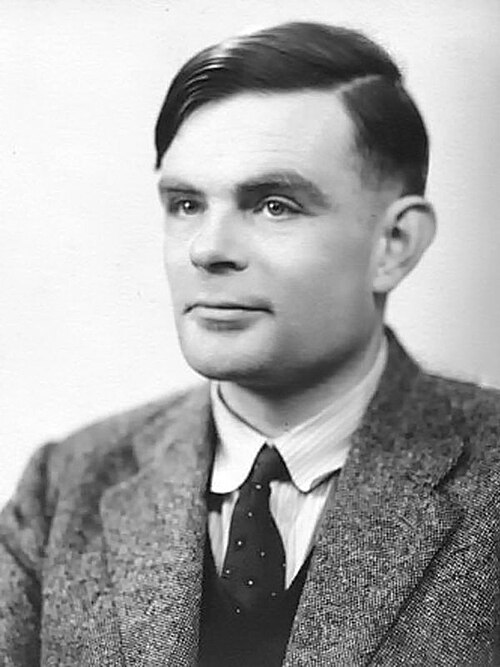
\includegraphics[
        width=0.78\linewidth,
        height=3.55cm,
        keepaspectratio
      ]{figures/hydra/Alan_Turing_(1951).jpg}

      \vspace{0.08cm}

      {\color{HydraGold}\bfseries\fontsize{18}{21}\selectfont
        1952\par}

      {\color{HydraWhite}\bfseries\fontsize{9.2}{11}\selectfont
        Alan Turing\par}

      \vspace{0.04cm}

      {\color{HydraMuted}\fontsize{6.6}{8.1}\selectfont
        \textit{The Chemical Basis of Morphogenesis}
      \par}
    \end{column}

    \begin{column}{0.67\textwidth}
      {\color{HydraWhite}\fontsize{12.6}{16}\selectfont
      \[
        \begin{aligned}
          \partial_tu&=D_u\Delta u+f(u,v)
          \\
          \partial_tv&=D_v\Delta v+g(u,v)
        \end{aligned}
      \]
      }

      \vspace{-0.10cm}

      \HydraPoint[HydraGold]
        {Stable reactions}
        {Without spatial transport, small perturbations return to the homogeneous equilibrium.}

      \vspace{0.32cm}

      \HydraPoint[HydraCyan]
        {Unstable reaction--diffusion system}
        {After diffusion is introduced, one nonconstant spatial mode can begin to grow.}

      \vspace{-0.20cm}

      {\color{HydraWhite}\bfseries\fontsize{13.2}{16.2}\selectfont
      \[
        \boxed{D_u\neq D_v}
      \]
      }

      \vspace{-0.24cm}

      {\color{HydraMuted}\fontsize{7.8}{9.5}\selectfont
        Unequal diffusion is essential for classical two-species Turing instability.
      \par}
    \end{column}

  \end{columns}

  \source{
    A.~M. Turing, \textit{Phil. Trans. R. Soc. B} 237 (1952), 37--72.
    Portrait: Elliott \& Fry, 1951, Wikimedia Commons.
  }

\end{frame}


\begin{frame}{Equal diffusion shifts every spatial mode toward stability}

  \vspace{-0.35cm}

  \begin{center}
    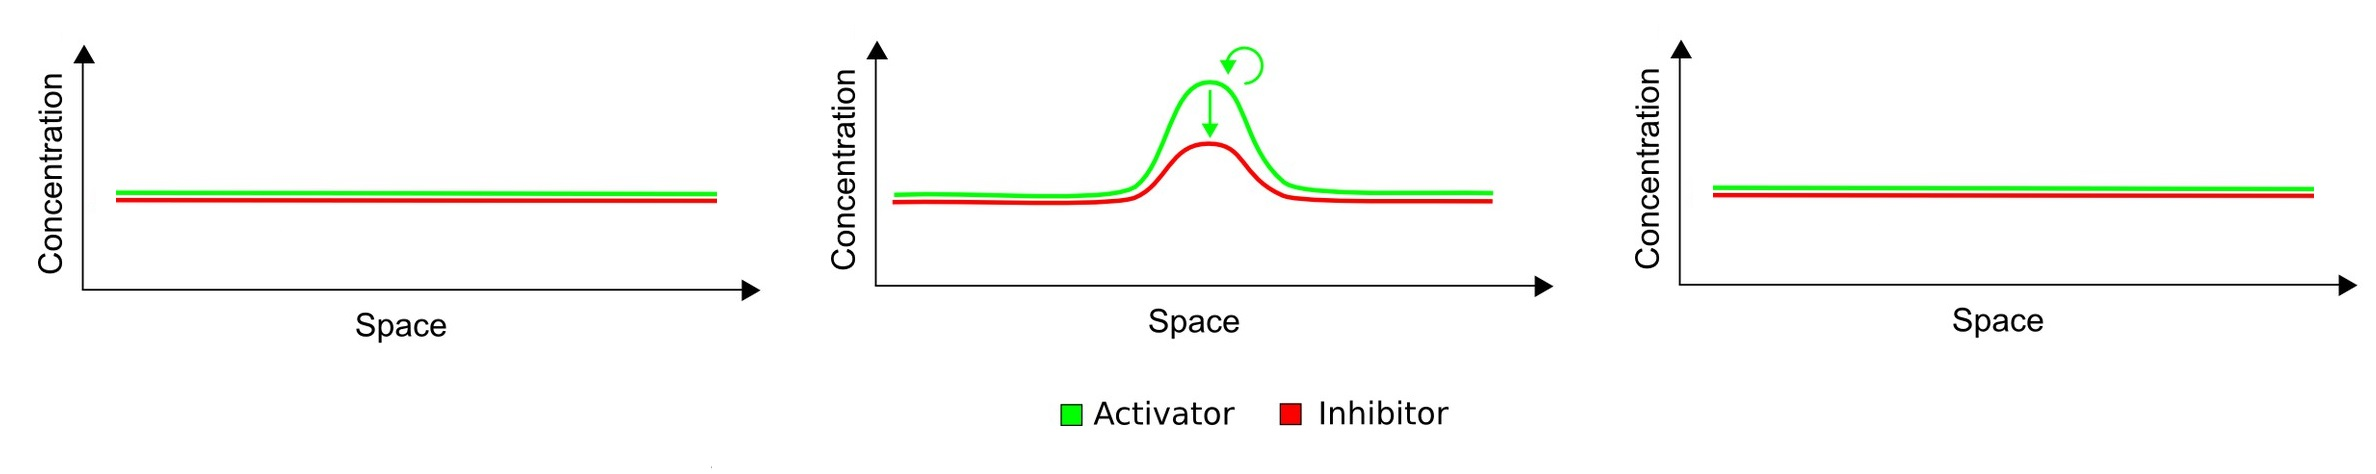
\includegraphics[
      width=0.98\textwidth,
      height=6.75cm,
      keepaspectratio
    ]{figures/turing/lax_14022_elife-14022-app3-fig1-v4.jpg}
  \end{center}

\end{frame}


\begin{frame}{Unequal diffusion can amplify a spatial mode}

  \vspace{-0.35cm}

  \begin{center}
    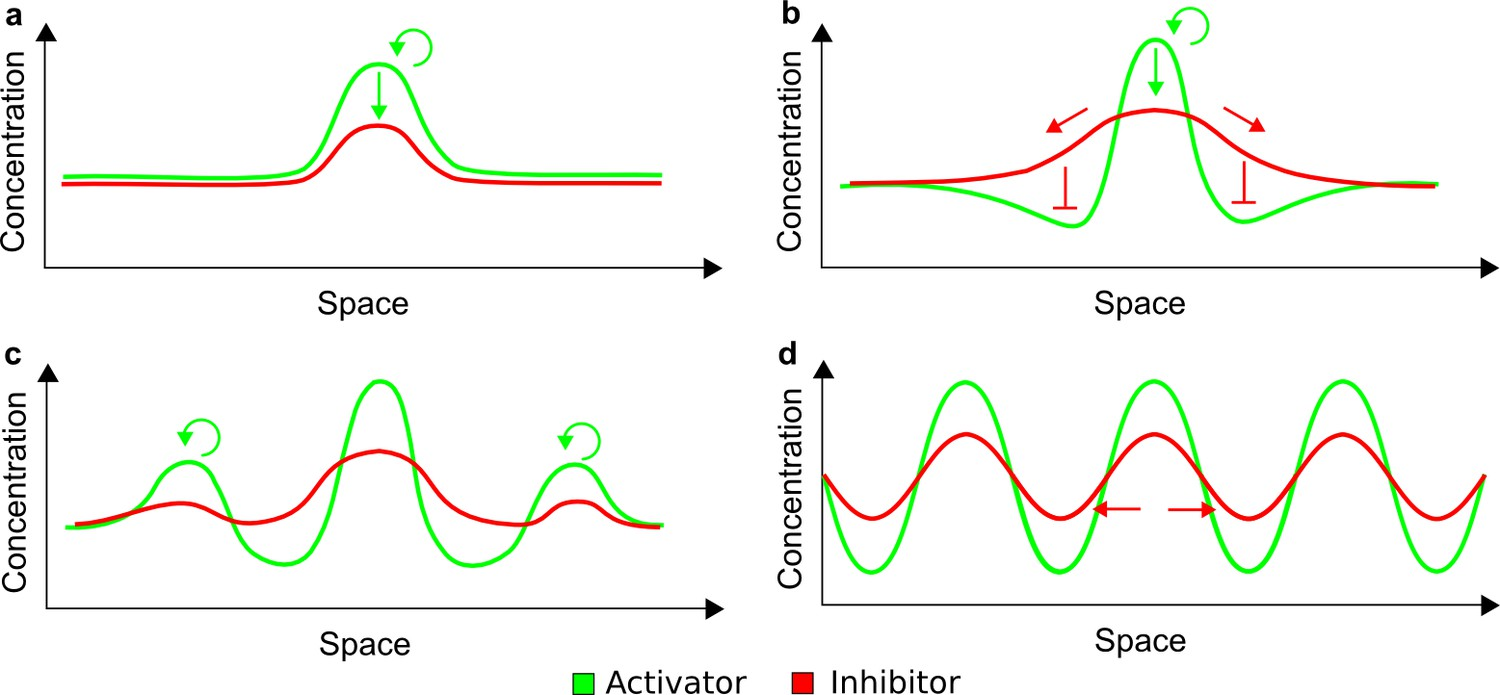
\includegraphics[
      width=0.98\textwidth,
      height=6.75cm,
      keepaspectratio
    ]{figures/turing/lax_14022_elife-14022-app3-fig1-v3.tif.jpg}
  \end{center}

\end{frame}





\HydraSubsection[
  \mbox{Linearization and spatial eigenfunctions}
  \mbox{reduce the PDE to one stability}
  \mbox{problem for each spatial mode}
]{Stability analysis}


\begin{frame}{The full reaction--diffusion problem}

  \vspace{-0.42cm}

  {\color{HydraWhite}\fontsize{8.4}{10.3}\selectfont
    Let $\Omega\subset\mathbb R^n$ be a bounded domain
  \par}

  \vspace{-0.26cm}

  {\color{HydraWhite}\fontsize{9.8}{12.4}\selectfont
  \begin{align*}
    \partial_tu
    &=D_u\Delta u+f(u,v)
    &&x\in\Omega
    \quad t>0
    \\
    \partial_tv
    &=D_v\Delta v+g(u,v)
    &&x\in\Omega
    \quad t>0
  \end{align*}
  }

  \vspace{0.16cm}

  {\color{HydraWhite}\fontsize{8.4}{10.3}\selectfont
    Initial conditions\par}

  \vspace{-0.28cm}

  {\color{HydraWhite}\fontsize{9.3}{11.7}\selectfont
  \begin{align*}
    u(x,0)&=u_0(x)
    &
    v(x,0)&=v_0(x)
    &&x\in\Omega
  \end{align*}
  }

  \vspace{-0.38cm}

  {\color{HydraWhite}\fontsize{8.4}{10.3}\selectfont
    Homogeneous Neumann boundary conditions\par}

  \vspace{-0.28cm}

  {\color{HydraWhite}\fontsize{9.3}{11.7}\selectfont
  \begin{align*}
    \nabla u\cdot\mathbf n
    &=0
    &
    \nabla v\cdot\mathbf n
    &=0
    &&x\in\partial\Omega
  \end{align*}
  }

  \vspace{-0.28cm}

  \begin{columns}[T,onlytextwidth]

    \begin{column}{0.56\textwidth}
      {\color{HydraGold}\fontsize{10}{10}\selectfont
        $\bullet$
      }
      {\color{HydraMuted}\fontsize{7.4}{9}\selectfont
        $f,g\in C^1(\mathbb R^2)$ describe local production,
        degradation and interactions at each spatial position
      }
    \end{column}

    \begin{column}{0.40\textwidth}
      {\color{HydraCyan}\fontsize{10}{10}\selectfont
        $\bullet$
      }
      {\color{HydraMuted}\fontsize{7.4}{9}\selectfont
        $D_u,D_v>0$ are the diffusion coefficients
      }
    \end{column}

  \end{columns}

\end{frame}


\begin{frame}{Homogeneous steady state}

  \vspace{-0.08cm}

  \begin{columns}[c,onlytextwidth]

    \begin{column}{0.58\textwidth}
      {\color{HydraGold}\bfseries\fontsize{7.6}{9.2}\selectfont
        HOMOGENEOUS EQUILIBRIUM\par}

      \vspace{-0.16cm}

      {\color{HydraWhite}\fontsize{11.6}{14.8}\selectfont
      \[
        \begin{pmatrix}
          u(x,t)\\
          v(x,t)
        \end{pmatrix}
        =
        \begin{pmatrix}
          \bar u\\
          \bar v
        \end{pmatrix}
      \]
      }

      \vspace{-0.22cm}

      {\color{HydraWhite}\fontsize{10.4}{13.2}\selectfont
      \[
        f(\bar u,\bar v)=0
        \qquad
        g(\bar u,\bar v)=0
      \]
      }

      \vspace{-0.18cm}

      {\color{HydraGold}\bfseries\fontsize{7.6}{9.2}\selectfont
        LOCAL JACOBIAN\par}

      \vspace{-0.16cm}

      {\color{HydraWhite}\fontsize{10.4}{13.2}\selectfont
      \[
        J(\bar u,\bar v)=
        \begin{pmatrix}
          f_u(\bar u,\bar v)&f_v(\bar u,\bar v)\\
          g_u(\bar u,\bar v)&g_v(\bar u,\bar v)
        \end{pmatrix}
      \]
      }

      \vspace{-0.08cm}

      {\color{HydraMuted}\fontsize{7.5}{9.1}\selectfont
        Both eigenvalues of $J(\bar u,\bar v)$ have negative real parts
      \par}

      \vspace{-0.18cm}

      {\color{HydraWhite}\bfseries\fontsize{11.6}{14.5}\selectfont
      \[
        \boxed{
          \operatorname{tr}J(\bar u,\bar v)<0
          \qquad
          \det J(\bar u,\bar v)>0
        }
      \]
      }
    \end{column}

    \begin{column}{0.38\textwidth}
      \centering

      % REPLACEABLE VISUAL
      % Replace the tikzpicture with:
      % \includegraphics[width=\linewidth,height=4.90cm,keepaspectratio]{figures/turing/...}
      \begin{tikzpicture}[x=0.88cm,y=0.88cm]
        \draw[-{Latex[length=2.2mm]},HydraMuted,line width=0.75pt]
          (0.35,0.55) -- (5.65,0.55)
          node[below,text=HydraMuted,font=\fontsize{7}{8.2}\selectfont] {$x$};

        \draw[HydraGold,line width=1.55pt] (0.55,3.95) -- (5.35,3.95);
        \draw[HydraCyan,line width=1.55pt] (0.55,2.15) -- (5.35,2.15);

        \node[anchor=west,text=HydraGold,
          font=\bfseries\fontsize{8}{9.5}\selectfont]
          at (0.55,4.25) {$u(x)=\bar u$};
        \node[anchor=west,text=HydraCyan,
          font=\bfseries\fontsize{8}{9.5}\selectfont]
          at (0.55,2.45) {$v(x)=\bar v$};

        \foreach \x in {0.65,1.45,...,5.25}{
          \fill[HydraGold] (\x,3.95) circle[radius=0.045cm];
          \fill[HydraCyan] (\x,2.15) circle[radius=0.045cm];
        }

        \node[anchor=north,text=HydraMuted,text width=4.9cm,align=center,
          font=\fontsize{7.2}{8.8}\selectfont]
          at (2.95,1.25)
          {the same concentrations at every position};
      \end{tikzpicture}

      \vspace{-0.12cm}

      \HydraPoint[HydraCyan]
        {Stable without spatial variation}
        {The reaction kinetics restore every sufficiently small homogeneous perturbation.}
    \end{column}

  \end{columns}

\end{frame}


\begin{frame}{Perturb both concentrations around the steady state}

  \vspace{-0.44cm}

  \begin{columns}[T,onlytextwidth]

    \begin{column}{0.40\textwidth}
      {\color{HydraGold}\bfseries\fontsize{7.6}{9.2}\selectfont
        SMALL PERTURBATION\par}

      \vspace{-0.28cm}

      {\color{HydraWhite}\fontsize{9.5}{12}\selectfont
      \begin{align*}
        u(x,t)&=\bar u+\eta(x,t)
        \\
        v(x,t)&=\bar v+\xi(x,t)
      \end{align*}
      }

      \vspace{-0.42cm}

      % REPLACEABLE VISUAL
      % Replace the tikzpicture with:
      % \includegraphics[width=\linewidth,height=2.20cm,keepaspectratio]{figures/turing/...}
      \begin{tikzpicture}[x=0.72cm,y=0.68cm]
        \draw[-{Latex[length=2mm]},HydraMuted,line width=0.7pt]
          (0.35,0.45) -- (6.20,0.45)
          node[below,text=HydraMuted,font=\fontsize{6.8}{8}\selectfont] {$x$};
        \draw[HydraLine,line width=0.65pt] (0.45,2.20) -- (5.95,2.20);
        \draw[HydraGold,line width=1.35pt,domain=0.45:5.95,samples=100]
          plot (\x,{2.20+0.18*cos(360*2*(\x-0.45)/5.50)});
        \draw[HydraCyan,line width=1.30pt,domain=0.45:5.95,samples=100]
          plot (\x,{1.15+0.13*cos(360*2*(\x-0.45)/5.50)});
        \draw[HydraLine,line width=0.65pt] (0.45,1.15) -- (5.95,1.15);
        \node[anchor=west,text=HydraGold,
          font=\fontsize{7}{8.4}\selectfont] at (4.85,2.58) {$\eta$};
        \node[anchor=west,text=HydraCyan,
          font=\fontsize{7}{8.4}\selectfont] at (4.85,1.48) {$\xi$};
      \end{tikzpicture}
    \end{column}

    \begin{column}{0.56\textwidth}
      {\color{HydraMuted}\fontsize{7.7}{9.4}\selectfont
        Expand both reaction terms around $(\bar u,\bar v)$
      \par}

      \vspace{-0.30cm}

      {\color{HydraWhite}\fontsize{7.2}{8.9}\selectfont
      \begin{align*}
        f(\bar u+\eta,\bar v+\xi)
        &=f(\bar u,\bar v)
        +f_u(\bar u,\bar v)\eta
        +f_v(\bar u,\bar v)\xi
        +O\!\left(\lVert(\eta,\xi)\rVert^2\right)
        \\
        g(\bar u+\eta,\bar v+\xi)
        &=g(\bar u,\bar v)
        +g_u(\bar u,\bar v)\eta
        +g_v(\bar u,\bar v)\xi
        +O\!\left(\lVert(\eta,\xi)\rVert^2\right)
      \end{align*}
      }

      \vspace{-0.34cm}

      {\color{HydraMuted}\fontsize{7.2}{8.8}\selectfont
        Since $(\bar u,\bar v)$ is constant and
        $f(\bar u,\bar v)=g(\bar u,\bar v)=0$, substitution gives
      \par}

      \vspace{-0.32cm}

      {\color{HydraWhite}\fontsize{7.2}{8.9}\selectfont
      \begin{align*}
        \partial_t\eta
        &=D_u\Delta\eta
        +f_u(\bar u,\bar v)\eta
        +f_v(\bar u,\bar v)\xi
        +O\!\left(\lVert(\eta,\xi)\rVert^2\right)
        \\
        \partial_t\xi
        &=D_v\Delta\xi
        +g_u(\bar u,\bar v)\eta
        +g_v(\bar u,\bar v)\xi
        +O\!\left(\lVert(\eta,\xi)\rVert^2\right)
      \end{align*}
      }

    \end{column}

  \end{columns}

  \vspace{-0.14cm}

  {\color{HydraMuted}\fontsize{7.7}{9.4}\selectfont
    For infinitesimal perturbations, keep only first-order terms
  \par}

  \vspace{-0.30cm}

  {\color{HydraWhite}\bfseries\fontsize{9.2}{11.6}\selectfont
  \begin{align*}
    \boxed{
      \partial_t
      \begin{pmatrix}
        \eta\\
        \xi
      \end{pmatrix}
      =
      J(\bar u,\bar v)
      \begin{pmatrix}
        \eta\\
        \xi
      \end{pmatrix}
      +
      \begin{pmatrix}
        D_u&0\\
        0&D_v
      \end{pmatrix}
      \Delta
      \begin{pmatrix}
        \eta\\
        \xi
      \end{pmatrix}
    }
  \end{align*}
  }

\end{frame}


\begin{frame}{Spatial eigenfunctions separate the perturbation}

  \vspace{-0.08cm}

  \begin{columns}[c,onlytextwidth]

    \begin{column}{0.56\textwidth}
      {\color{HydraMuted}\fontsize{7.8}{9.6}\selectfont
        Use the eigenfunctions introduced in the diffusion section
      \par}

      \vspace{-0.16cm}

      {\color{HydraWhite}\fontsize{10.6}{13.5}\selectfont
      \[
        -\Delta\phi_k=\mu_k\phi_k
        \qquad
        \nabla\phi_k\cdot n=0
        \quad\text{on }\partial\Omega
      \]
      }

      \vspace{-0.18cm}

      {\color{HydraWhite}\fontsize{10.2}{13}\selectfont
      \[
        \begin{pmatrix}
          \eta(x,t)\\
          \xi(x,t)
        \end{pmatrix}
        =
        \sum_{k=0}^{\infty}
        \begin{pmatrix}
          a_k(t)\\
          b_k(t)
        \end{pmatrix}
        \phi_k(x)
      \]
      }

      \vspace{-0.14cm}

      \HydraPoint[HydraGold]
        {One spatial shape}
        {$\phi_k(x)$ determines where the perturbation is positive and negative.}

      \vspace{-0.06cm}

      \HydraPoint[HydraCyan]
        {Two chemical amplitudes}
        {$a_k(t)$ and $b_k(t)$ determine how strongly that shape appears in each substance.}
    \end{column}

    \begin{column}{0.40\textwidth}
      \centering

      % REPLACEABLE VISUAL
      % Replace the tikzpicture with:
      % \includegraphics[width=\linewidth,height=4.95cm,keepaspectratio]{figures/turing/...}
      \begin{tikzpicture}[x=0.84cm,y=0.86cm]
        \foreach \y/\n in {
          4.55/0,
          3.20/1,
          1.85/2,
          0.50/3
        }{
          \draw[HydraLine,line width=0.55pt] (0.50,\y) -- (6.10,\y);
          \node[anchor=east,text=HydraMuted,
            font=\fontsize{7}{8.4}\selectfont]
            at (0.32,\y) {$k=\n$};
        }

        \draw[HydraWhite,line width=1.35pt] (0.50,4.73) -- (6.10,4.73);
        \draw[HydraGold,line width=1.35pt,domain=0.50:6.10,samples=100]
          plot (\x,{3.20+0.28*cos(180*(\x-0.50)/5.60)});
        \draw[HydraCyan,line width=1.35pt,domain=0.50:6.10,samples=100]
          plot (\x,{1.85+0.28*cos(360*(\x-0.50)/5.60)});
        \draw[HydraViolet,line width=1.35pt,domain=0.50:6.10,samples=100]
          plot (\x,{0.50+0.28*cos(540*(\x-0.50)/5.60)});
      \end{tikzpicture}

      \vspace{-0.05cm}

      {\color{HydraMuted}\fontsize{7.4}{9}\selectfont
        Each spatial shape will evolve independently after linearization.
      \par}
    \end{column}

  \end{columns}

\end{frame}


\begin{frame}{Each mode is a two-dimensional stability problem}

  \vspace{-0.26cm}

  {\color{HydraMuted}\fontsize{7.4}{9}\selectfont
    Combining the linearized perturbation equation with the eigenfunction expansion
  \par}

  \vspace{-0.12cm}

  \begin{columns}[c,onlytextwidth]

    \begin{column}{0.57\textwidth}
      {\color{HydraWhite}\fontsize{7.5}{9.3}\selectfont
      \begin{align*}
        \partial_t
        \begin{pmatrix}
          \eta\\
          \xi
        \end{pmatrix}
        &=
        J(\bar u,\bar v)
        \begin{pmatrix}
          \eta\\
          \xi
        \end{pmatrix}
        +
        \begin{pmatrix}
          D_u&0\\
          0&D_v
        \end{pmatrix}
        \Delta
        \begin{pmatrix}
          \eta\\
          \xi
        \end{pmatrix}
      \end{align*}
      }
    \end{column}

    \begin{column}{0.04\textwidth}
      \centering
      {\color{HydraGold}\bfseries\fontsize{15}{15}\selectfont
        $+$
      }
    \end{column}

    \begin{column}{0.35\textwidth}
      {\color{HydraWhite}\fontsize{7.9}{9.8}\selectfont
      \begin{align*}
        \begin{pmatrix}
          \eta(x,t)\\
          \xi(x,t)
        \end{pmatrix}
        &=
        \sum_{k=0}^{\infty}
        \begin{pmatrix}
          a_k(t)\\
          b_k(t)
        \end{pmatrix}
        \phi_k(x)
      \end{align*}
      }
    \end{column}

  \end{columns}

  \vspace{0.14cm}

  \begin{columns}[c,onlytextwidth]
    \begin{column}{0.57\textwidth}
      \mbox{}
    \end{column}

    \begin{column}{0.04\textwidth}
      \centering
      {\color{HydraCyan}\fontsize{15}{15}\selectfont
        $\Downarrow$
      }
    \end{column}

    \begin{column}{0.35\textwidth}
      \mbox{}
    \end{column}
  \end{columns}

  \vspace{0.14cm}

  {\color{HydraWhite}\fontsize{7.7}{9.6}\selectfont
  \begin{align*}
    \sum_{k=0}^{\infty}
    \frac{d}{dt}
    \binom{a_k}{b_k}
    \phi_k
    &=
    J(\bar u,\bar v)
    \sum_{k=0}^{\infty}
    \binom{a_k}{b_k}
    \phi_k
    +
    \begin{pmatrix}
      D_u&0\\
      0&D_v
    \end{pmatrix}
    \sum_{k=0}^{\infty}
    \binom{a_k}{b_k}
    \Delta\phi_k
  \end{align*}
  }

  \vspace{-0.30cm}

  {\color{HydraMuted}\fontsize{7.4}{9}\selectfont
    Since $\Delta\phi_k=-\mu_k\phi_k$ and
    $\{\phi_k\}_{k=0}^{\infty}$ is an orthonormal basis,
    the coefficients of every $\phi_k$ must agree
  \par}

  \vspace{-0.20cm}

  {\color{HydraWhite}\bfseries\fontsize{9.4}{11.8}\selectfont
  \begin{align*}
    \boxed{
      \frac{d}{dt}
      \binom{a_k}{b_k}
      =
      \left(
        J(\bar u,\bar v)-\mu_k
        \begin{pmatrix}
          D_u&0\\
          0&D_v
        \end{pmatrix}
      \right)
      \binom{a_k}{b_k}
    }
  \end{align*}
  }

\end{frame}


\begin{frame}{Define the stability matrix of each mode}

  \vspace{-0.46cm}

  {\color{HydraWhite}\fontsize{9.2}{11.6}\selectfont
  \begin{align*}
    \frac{d}{dt}
    \binom{a_k}{b_k}
    =
    \left(
      J(\bar u,\bar v)-\mu_k
      \begin{pmatrix}
        D_u&0\\
        0&D_v
      \end{pmatrix}
    \right)
    \binom{a_k}{b_k}
  \end{align*}
  }

  \vspace{-0.30cm}

  {\color{HydraMuted}\fontsize{7.6}{9.2}\selectfont
    Define the stability matrix associated with the $k$th spatial mode
  \par}

  \vspace{-0.24cm}

  {\color{HydraWhite}\fontsize{8.7}{10.9}\selectfont
  \begin{align*}
    \boxed{
      \begin{aligned}
        M_k
        =
        J(\bar u,\bar v)-\mu_k
        \begin{pmatrix}
          D_u&0\\
          0&D_v
        \end{pmatrix}&=
        \begin{pmatrix}
          f_u(\bar u,\bar v)-D_u\mu_k
          &f_v(\bar u,\bar v)
          \\
          g_u(\bar u,\bar v)
          &g_v(\bar u,\bar v)-D_v\mu_k
        \end{pmatrix}
      \end{aligned}
    }
  \end{align*}
  }

  \vspace{-0.34cm}

  {\color{HydraWhite}\bfseries\fontsize{11.2}{14}\selectfont
  \begin{align*}
    \boxed{
      \frac{d}{dt}
      \binom{a_k}{b_k}
      =
      M_k
      \binom{a_k}{b_k}
    }
  \end{align*}
  }

  \vspace{-0.28cm}

  \HydraTakeaway{
    Every spatial wavelength has its own $2\times2$ stability matrix
  }

\end{frame}


\begin{frame}{The homogeneous mode remains locally stable}

  \vspace{-0.08cm}

  \begin{columns}[c,onlytextwidth]

    \begin{column}{0.47\textwidth}
      {\color{HydraGold}\bfseries\fontsize{8}{9.5}\selectfont
        HOMOGENEOUS MODE\par}

      \vspace{-0.12cm}

      {\color{HydraWhite}\fontsize{12}{15.2}\selectfont
      \[
        \phi_0(x)=\text{constant}
        \qquad
        \mu_0=0
      \]
      }

      \vspace{-0.20cm}

      {\color{HydraWhite}\bfseries\fontsize{13.2}{16.2}\selectfont
      \[
        \boxed{M_0=J(\bar u,\bar v)}
      \]
      }

      \vspace{-0.14cm}

      % REPLACEABLE VISUAL
      \begin{tikzpicture}[x=0.82cm,y=0.82cm]
        \draw[HydraLine,line width=0.6pt] (0.35,1.35) -- (6.35,1.35);
        \draw[HydraGold,line width=1.5pt] (0.35,2.15) -- (6.35,2.15);
        \node[anchor=north,text=HydraMuted,
          font=\fontsize{7.2}{8.7}\selectfont]
          at (3.35,0.98) {the same perturbation everywhere};
      \end{tikzpicture}

      \vspace{-0.10cm}

      \HydraPoint[HydraCyan]
        {Stable by assumption}
        {The local reaction analysis already guarantees decay of this mode.}
    \end{column}

    \begin{column}{0.04\textwidth}
      \centering
      {\color{HydraLine}\rule{0.7pt}{5.1cm}}
    \end{column}

    \begin{column}{0.45\textwidth}
      {\color{HydraCyan}\bfseries\fontsize{8}{9.5}\selectfont
        NONCONSTANT MODES\par}

      \vspace{-0.12cm}

      {\color{HydraWhite}\fontsize{12}{15.2}\selectfont
      \[
        \mu_k>0
        \qquad
        k\geq1
      \]
      }

      \vspace{-0.20cm}

      {\color{HydraWhite}\fontsize{10.2}{13}\selectfont
      \[
        M_k
        =
        J(\bar u,\bar v)-\mu_k
        \begin{pmatrix}
          D_u&0\\
          0&D_v
        \end{pmatrix}
      \]
      }

      \vspace{-0.16cm}

      % REPLACEABLE VISUAL
      \begin{tikzpicture}[x=0.82cm,y=0.82cm]
        \draw[HydraLine,line width=0.6pt] (0.35,1.35) -- (6.35,1.35);
        \draw[HydraCyan,line width=1.5pt,domain=0.35:6.35,samples=100]
          plot (\x,{1.35+0.55*cos(360*2*(\x-0.35)/6.00)});
        \node[anchor=north,text=HydraMuted,
          font=\fontsize{7.2}{8.7}\selectfont]
          at (3.35,0.60) {a spatial pattern can change stability};
      \end{tikzpicture}

      \vspace{-0.10cm}

      \HydraPoint[HydraGold]
        {The Turing question}
        {Can any $M_k$ acquire an eigenvalue with positive real part?}
    \end{column}

  \end{columns}

\end{frame}


\begin{frame}{Diffusion makes the trace more negative}

  \vspace{-0.08cm}

  \begin{columns}[c,onlytextwidth]

    \begin{column}{0.57\textwidth}
      {\color{HydraWhite}\fontsize{10.2}{13}\selectfont
      \begin{align*}
        M_k
        =
        \begin{pmatrix}
          f_u(\bar u,\bar v)-D_u\mu_k&f_v(\bar u,\bar v)\\
          g_u(\bar u,\bar v)&g_v(\bar u,\bar v)-D_v\mu_k
        \end{pmatrix}
      \end{align*}
      }

      \vspace{-0.20cm}

      {\color{HydraWhite}\bfseries\fontsize{12.2}{15.2}\selectfont
      \begin{align*}
        \boxed{
          \operatorname{tr}(M_k)
          =
          \operatorname{tr}J(\bar u,\bar v)
          -
          (D_u+D_v)\mu_k
        }
      \end{align*}
      }

      \vspace{-0.16cm}

      \HydraPoint[HydraCyan]
        {The trace starts negative}
        {$\mu_0=0$ and $\operatorname{tr}(M_0)=\operatorname{tr}J(\bar u,\bar v)<0$ because the homogeneous equilibrium is locally stable.}

      \vspace{0.12cm}

      \HydraPoint[HydraGold]
        {Diffusion decreases it further}
        {For every $k\geq1$, the term $-(D_u+D_v)\mu_k$ is strictly negative.}

      \vspace{-0.08cm}

      {\color{HydraMuted}\fontsize{7.8}{9.5}\selectfont
        Therefore a Turing instability cannot occur through the trace becoming positive.
      \par}
    \end{column}

    \begin{column}{0.39\textwidth}
      \centering

      % REPLACEABLE VISUAL
      % Replace the tikzpicture with:
      % \includegraphics[width=\linewidth,height=4.80cm,keepaspectratio]{figures/turing/...}
      \begin{tikzpicture}[x=0.88cm,y=0.88cm]
        \draw[-{Latex[length=2.2mm]},HydraMuted,line width=0.75pt]
          (0.45,3.60) -- (5.70,3.60)
          node[below,text=HydraMuted,font=\fontsize{7}{8.2}\selectfont] {$\mu_k$};
        \draw[-{Latex[length=2.2mm]},HydraMuted,line width=0.75pt]
          (0.65,0.40) -- (0.65,5.15)
          node[left,text=HydraMuted,font=\fontsize{7}{8.2}\selectfont] {$\operatorname{tr}(M_k)$};

        \draw[HydraGold,line width=1.65pt]
          (0.65,2.95) -- (5.25,0.72);

        \fill[HydraWhite] (0.65,2.95) circle[radius=0.075cm];
        \foreach \x/\lab in {1.45/1,2.35/2,3.35/3,4.55/4}{
          \pgfmathsetmacro{\yy}{2.95-0.4848*(\x-0.65)}
          \fill[HydraCyan] (\x,\yy) circle[radius=0.070cm];
          \node[anchor=north,text=HydraMuted,
            font=\fontsize{6.4}{7.7}\selectfont]
            at (\x,3.50) {$\mu_{\lab}$};
        }
        \node[anchor=north,text=HydraMuted,
          font=\fontsize{6.4}{7.7}\selectfont]
          at (0.48,3.50) {$\mu_0$};

        \node[anchor=east,text=HydraWhite,
          font=\fontsize{7.2}{8.7}\selectfont]
          at (0.48,3.02) {$\operatorname{tr}J(\bar u,\bar v)<0$};

        \node[anchor=west,text=HydraGold,
          font=\bfseries\fontsize{7.4}{8.9}\selectfont]
          at (2.95,1.92) {$\operatorname{tr}(M_k)$};

        \fill[HydraRed,opacity=0.05] (0.65,0.42) rectangle (5.55,3.58);
        \node[text=HydraMuted,font=\fontsize{7.2}{8.7}\selectfont]
          at (3.45,4.45) {zero is never crossed};
      \end{tikzpicture}
    \end{column}

  \end{columns}

\end{frame}


\begin{frame}{The determinant contains the instability mechanism}

  \vspace{-0.08cm}

  {\color{HydraMuted}\fontsize{7.7}{9.4}\selectfont
    Compute the determinant of the mode matrix
  \par}

  \vspace{-0.16cm}

  {\color{HydraWhite}\fontsize{10}{12.7}\selectfont
  \begin{align*}
    \det(M_k)
    &=
    \det
    \begin{pmatrix}
      f_u(\bar u,\bar v)-D_u\mu_k&f_v(\bar u,\bar v)\\
      g_u(\bar u,\bar v)&g_v(\bar u,\bar v)-D_v\mu_k
    \end{pmatrix}
    \\
    &=
    \left(f_u(\bar u,\bar v)-D_u\mu_k\right)
    \left(g_v(\bar u,\bar v)-D_v\mu_k\right)
    -f_v(\bar u,\bar v)g_u(\bar u,\bar v)
    \\
    &=
    \det J(\bar u,\bar v)
    -
    \left(D_vf_u(\bar u,\bar v)+D_ug_v(\bar u,\bar v)\right)\mu_k
    +
    D_uD_v\mu_k^2
  \end{align*}
  }

  \vspace{-0.32cm}

  {\color{HydraWhite}\bfseries\fontsize{10.4}{13.2}\selectfont
  \begin{align*}
    {\color{HydraGold}
      \boxed{
        \det(M_k)
        =
        \det J(\bar u,\bar v)-A\mu_k+D_uD_v\mu_k^2
      }
    }
    \qquad
    A=D_vf_u(\bar u,\bar v)+D_ug_v(\bar u,\bar v)
  \end{align*}
  }

  \vspace{-0.14cm}

  \begin{columns}[T,onlytextwidth]
    \begin{column}{0.31\textwidth}
      \HydraPoint[HydraCyan]
        {Positive at $\mu_0=0$}
        {$\det(M_0)=\det J(\bar u,\bar v)>0$ follows from local stability.}
    \end{column}

    \begin{column}{0.31\textwidth}
      \HydraPoint[HydraGold]
        {The linear term can decrease it}
        {Unequal diffusion weights $f_u$ and $g_v$ differently inside $A$.}
    \end{column}

    \begin{column}{0.31\textwidth}
      \HydraPoint[HydraGold]
        {Very short waves are stable}
        {$D_uD_v\mu_k^2$ dominates for sufficiently large $k$.}
    \end{column}
  \end{columns}

\end{frame}


\begin{frame}{Turing instability condition}

  \vspace{-0.24cm}

  \begin{columns}[c,onlytextwidth]

    \begin{column}{0.57\textwidth}

      \vspace{-0.30cm}

      {\color{HydraWhite}\bfseries\fontsize{10.4}{13.2}\selectfont
      \begin{align*}
        {\color{HydraGold}
          \boxed{
            \det(M_k)
            =
            \det J(\bar u,\bar v)-A\mu_k+D_uD_v\mu_k^2
          }
        }
      \end{align*}
      }

      \vspace{-0.44cm}

      \HydraPoint[HydraCyan]
        {$\det(M_k)>0$}
        {The $k$th spatial mode is stable.}

      \vspace{-0.0cm}

      \HydraPoint[HydraGold]
        {$\det(M_k)<0$}
        {The $k$th spatial mode is unstable.}

      \vspace{-0.3cm}

{\color{HydraWhite}\fontsize{9.5}{12}\selectfont
      \begin{align*}
        \det(M_k)<0
        \quad\Longleftrightarrow\quad
        \mu_-<\mu_k<\mu_+
      \end{align*}
      }

      \vspace{-0.3cm}
      {\color{HydraMuted}\fontsize{7.4}{9.1}\selectfont
        A negative interval exists when
      \par}

      \vspace{-0.62cm}

      {\color{HydraWhite}\fontsize{9.5}{12}\selectfont
      \begin{align*}
        A>0
        \qquad
        A^2>4D_uD_v\det J(\bar u,\bar v)
      \end{align*}
      }

      \vspace{-0.80cm}

      {\color{HydraWhite}\fontsize{8.8}{11.1}\selectfont
      \begin{align*}
        \mu_\pm
        =
        \frac{
          A\pm\sqrt{A^2-4D_uD_v\det J(\bar u,\bar v)}
        }{
          2D_uD_v
        }
      \end{align*}
      }
    \end{column}

    \begin{column}{0.39\textwidth}
      \centering

      % REPLACEABLE VISUAL
      % Replace the tikzpicture with:
      % \includegraphics[width=\linewidth,height=4.95cm,keepaspectratio]{figures/turing/...}
      \begin{tikzpicture}[x=0.88cm,y=0.88cm]
        \fill[HydraGold,opacity=0.10]
          plot[domain=1.75:4.55,samples=100]
            (\x,{2.35+0.52*(\x-1.75)*(\x-4.55)})
          -- (4.55,2.35) -- (1.75,2.35) -- cycle;

        \draw[-{Latex[length=2.2mm]},HydraMuted,line width=0.75pt]
          (0.40,2.35) -- (5.90,2.35)
          node[below,text=HydraMuted,font=\fontsize{7}{8.2}\selectfont] {$\mu_k$};
        \draw[-{Latex[length=2.2mm]},HydraMuted,line width=0.75pt]
          (0.65,0.45) -- (0.65,5.25)
          node[left,text=HydraMuted,font=\fontsize{7}{8.2}\selectfont] {$\det(M_k)$};

        \draw[HydraGold,line width=1.75pt,domain=0.65:5.55,samples=100]
          plot (\x,{2.35+0.52*(\x-1.75)*(\x-4.55)});

        \foreach \x/\lab/\col in {0.85/0/HydraWhite,1.40/1/HydraCyan,2.25/2/HydraGold,3.15/3/HydraGold,4.20/4/HydraGold,5.15/5/HydraCyan}{
          \pgfmathsetmacro{\yy}{2.35+0.52*(\x-1.75)*(\x-4.55)}
          \fill[\col] (\x,\yy) circle[radius=0.070cm];
          \node[anchor=south,text=HydraMuted,
            font=\fontsize{6.2}{7.5}\selectfont]
            at (\x,2.46) {$\mu_{\lab}$};
        }

        \fill[HydraWhite] (1.75,2.35) circle[radius=0.075cm];
        \fill[HydraWhite] (4.55,2.35) circle[radius=0.075cm];

        \node[anchor=north,text=HydraMuted,
          font=\fontsize{6.9}{8.3}\selectfont]
          at (1.75,2.22) {$\mu_-$};
        \node[anchor=north,text=HydraMuted,
          font=\fontsize{6.9}{8.3}\selectfont]
          at (4.55,2.22) {$\mu_+$};

        \node[text=HydraGold,font=\bfseries\fontsize{7.5}{9}\selectfont]
          at (3.15,0.88) {unstable band};
        \node[text=HydraMuted,font=\fontsize{7.1}{8.6}\selectfont]
          at (3.15,4.55) {stable};
      \end{tikzpicture}
    \end{column}

  \end{columns}

\end{frame}


\begin{frame}{Turing instability theorem}

  \vspace{-0.28cm}

  {\color{HydraWhite}\bfseries\fontsize{9.8}{12.5}\selectfont
  \begin{align*}
    \boxed{
      \begin{aligned}
        \partial_tu&=D_u\Delta u+f(u,v)
        \\
        \partial_tv&=D_v\Delta v+g(u,v)
      \end{aligned}
    }
  \end{align*}
  }

  \vspace{+0.34cm}

  {\color{HydraGold}\bfseries\fontsize{7.8}{9.4}\selectfont
    THEOREM\par}

  \vspace{0.14cm}

  {\color{HydraWhite}\fontsize{9.2}{12}\selectfont
    If the system is stable in the absence of diffusion, and $u$ satisfies the autocatalysis condition, i.e.
    $f_u(\bar u,\bar v)>0$, diffusion $D_u$ is sufficiently small and diffusion $D_v$ is
    sufficiently large, then diffusion destabilizes the homogeneous steady
    state $(\bar u,\bar v)$.
  \par}

\end{frame}


\HydraSubsection[
  \mbox{The unstable band must intersect}
  \mbox{the discrete spatial spectrum}
  \mbox{allowed by the tissue geometry}
]{Mode selection}


\begin{frame}{Only eigenvalues inside the unstable band can grow}

  \vspace{-0.08cm}

  \begin{columns}[c,onlytextwidth]
    \begin{column}{0.72\textwidth}
      \centering

      % REPLACEABLE VISUAL
      % Replace the tikzpicture with the user's unstable-eigenmodes figure:
      % \includegraphics[width=\linewidth,height=5.20cm,keepaspectratio]{figures/turing/...}
      \begin{tikzpicture}[x=1.02cm,y=0.92cm]
        \fill[HydraGold,opacity=0.10]
          plot[domain=1.75:4.55,samples=100]
            (\x,{2.35+0.52*(\x-1.75)*(\x-4.55)})
          -- (4.55,2.35) -- (1.75,2.35) -- cycle;

        \draw[-{Latex[length=2.3mm]},HydraMuted,line width=0.75pt]
          (0.40,2.35) -- (6.20,2.35)
          node[below,text=HydraMuted,font=\fontsize{7}{8.2}\selectfont] {$\mu_k$};
        \draw[-{Latex[length=2.3mm]},HydraMuted,line width=0.75pt]
          (0.65,0.30) -- (0.65,5.25)
          node[left,text=HydraMuted,font=\fontsize{7}{8.2}\selectfont] {$\det(M_k)$};

        \draw[HydraGold,line width=1.75pt,domain=0.65:5.65,samples=120]
          plot (\x,{2.35+0.52*(\x-1.75)*(\x-4.55)});

        \foreach \x/\lab/\col in {0.65/0/HydraCyan,1.25/1/HydraCyan,2.00/2/HydraGold,2.85/3/HydraGold,3.80/4/HydraGold,4.75/5/HydraCyan,5.50/6/HydraCyan}{
          \pgfmathsetmacro{\yy}{2.35+0.52*(\x-1.75)*(\x-4.55)}
          \fill[\col] (\x,\yy) circle[radius=0.085cm];
          \node[anchor=north,text=HydraMuted,
            font=\fontsize{6.6}{8}\selectfont]
            at (\x,{\yy-0.12}) {$\mu_{\lab}$};
        }

        \fill[HydraWhite] (1.75,2.35) circle[radius=0.070cm];
        \fill[HydraWhite] (4.55,2.35) circle[radius=0.070cm];
        \node[anchor=north,text=HydraMuted,
          font=\fontsize{6.6}{8}\selectfont]
          at (1.75,2.22) {$\mu_-$};
        \node[anchor=north,text=HydraMuted,
          font=\fontsize{6.6}{8}\selectfont]
          at (4.55,2.22) {$\mu_+$};

        \node[text=HydraGold,font=\bfseries\fontsize{7.6}{9.1}\selectfont]
          at (3.15,0.72) {growing eigenmodes};
      \end{tikzpicture}
    \end{column}

    \begin{column}{0.24\textwidth}
      \HydraPoint[HydraGold]
        {Only selected modes grow}
        {The unstable band is continuous, but the tissue supplies only discrete eigenvalues.}
    \end{column}
  \end{columns}

  \vspace{0.46cm}

  \begin{columns}[c,onlytextwidth]
    \begin{column}{0.19\textwidth}
      \centering
      {\color{HydraWhite}\bfseries\fontsize{10.2}{12.9}\selectfont
        $\det(M_k)<0$
      \par}
    \end{column}

    \begin{column}{0.07\textwidth}
      \centering
      {\color{HydraCyan}\fontsize{17}{17}\selectfont
        $\Rightarrow$
      \par}
    \end{column}

    \begin{column}{0.29\textwidth}
      \centering
      {\color{HydraWhite}\fontsize{8.2}{10.4}\selectfont
        Exists a positive eigenvalue $\lambda_{k,+}$ 
      \par}
    \end{column}

    \begin{column}{0.07\textwidth}
      \centering
      {\color{HydraCyan}\fontsize{17}{17}\selectfont
        $\Rightarrow$
      \par}
    \end{column}

    \begin{column}{0.30\textwidth}
      \centering
      {\color{HydraWhite}\fontsize{8.2}{10.4}\selectfont
        Spatial mode $k$ grows at rate $e^{\lambda_{k,+}t}$
      \par}
    \end{column}
  \end{columns}

\end{frame}


\begin{frame}{Diffusion changes which modes are unstable}

  \vspace{-0.08cm}

  \begin{columns}[c,onlytextwidth]

    \begin{column}{0.67\textwidth}
      \centering

      % REPLACEABLE VISUAL
      % Replace the tikzpicture with:
      % \includegraphics[width=\linewidth,height=5.25cm,keepaspectratio]{figures/turing/...}
      \begin{tikzpicture}[x=0.98cm,y=0.88cm]
        \draw[-{Latex[length=2.2mm]},HydraMuted,line width=0.75pt]
          (0.40,2.15) -- (6.45,2.15)
          node[below,text=HydraMuted,font=\fontsize{7}{8.2}\selectfont] {$\mu_k$};
        \draw[-{Latex[length=2.2mm]},HydraMuted,line width=0.75pt]
          (0.65,0.30) -- (0.65,5.45)
          node[left,text=HydraMuted,font=\fontsize{7}{8.2}\selectfont] {$\det(M_k)$};

        \begin{scope}
          \clip (0.40,0.30) rectangle (6.20,5.35);
          \draw[HydraGold,line width=1.65pt,domain=0.65:5.85,samples=120]
            plot (\x,{2.15+1.00*(\x-1.15)*(\x-3.65)});
          \draw[HydraCyan,line width=1.65pt,domain=0.65:5.85,samples=120]
            plot (\x,{2.15+0.228*(\x-2.05)*(\x-5.35)});
        \end{scope}

        \foreach \x/\lab in {
          0.75/0,
          1.45/1,
          2.25/2,
          3.15/3,
          4.15/4,
          5.25/5
        }{
          \fill[HydraWhite] (\x,2.15) circle[radius=0.055cm];
          \node[anchor=north,text=HydraMuted,
            font=\fontsize{6.5}{7.8}\selectfont]
            at (\x,2.02) {$\mu_{\lab}$};
        }

        \draw[HydraGold,line width=1.25pt] (4.85,5.02) -- (5.25,5.02);
        \node[anchor=west,text=HydraMuted,
          font=\fontsize{7}{8.4}\selectfont]
          at (5.38,5.02) {diffusion set A};
        \draw[HydraCyan,line width=1.25pt] (4.85,4.62) -- (5.25,4.62);
        \node[anchor=west,text=HydraMuted,
          font=\fontsize{7}{8.4}\selectfont]
          at (5.38,4.62) {diffusion set B};

        \draw[HydraGold,line width=2.2pt] (1.15,0.42) -- (3.65,0.42);
        \draw[HydraCyan,line width=2.2pt] (2.05,0.92) -- (5.35,0.92);
        \node[anchor=east,text=HydraGold,
          font=\fontsize{6.8}{8.2}\selectfont]
          at (1.02,0.42) {band A};
        \node[anchor=west,text=HydraCyan,
          font=\fontsize{6.8}{8.2}\selectfont]
          at (5.48,0.92) {band B};
      \end{tikzpicture}
    \end{column}

    \begin{column}{0.29\textwidth}
      \HydraPoint[HydraGold]
        {The band moves}
        {Changing $D_u$ and $D_v$ changes its location and width.}

      \vspace{0.10cm}

      \HydraPoint[HydraCyan]
        {The selected modes change}
        {A different set of the fixed eigenvalues $\mu_k$ can become unstable.}

      \vspace{0.04cm}

      {\color{HydraMuted}\fontsize{7.5}{9.1}\selectfont
        Diffusion therefore controls the preferred spatial scale.
      \par}
    \end{column}

  \end{columns}

  \vspace{-0.24cm}

  \begin{columns}[c,onlytextwidth]
    \begin{column}{0.67\textwidth}
      \centering
      {\color{HydraWhite}\fontsize{9.4}{12}\selectfont
      \begin{align*}
        \det(M_k)
        =
        \det J(\bar u,\bar v)-A\mu_k+D_uD_v\mu_k^2
      \end{align*}
      }
    \end{column}

    \begin{column}{0.29\textwidth}
    \end{column}
  \end{columns}

\end{frame}


\begin{frame}{Diffusion and domain size}

  \vspace{-0.08cm}

  \begin{columns}[c,onlytextwidth]

    \begin{column}{0.54\textwidth}
      {\color{HydraMuted}\fontsize{7.4}{9.1}\selectfont
        Let $\widetilde\Omega$ be a fixed reference domain and scale it by $L>0$
      \par}

      \vspace{-0.34cm}

      {\color{HydraWhite}\fontsize{9.8}{12.5}\selectfont
      \begin{align*}
        \Omega_L=L\widetilde\Omega
        \qquad
        x=L\widetilde x
      \end{align*}
      }

      \vspace{-0.46cm}

      {\color{HydraMuted}\fontsize{7.4}{9.1}\selectfont
        Under the change of variables $x=L\widetilde x$, the system is
        equivalently written on the reference domain as
      \par}

      \vspace{-0.34cm}

      {\color{HydraWhite}\fontsize{8.4}{10.7}\selectfont
      \begin{align*}
        \partial_t\widetilde u
        &=
        \frac{D_u}{L^2}\Delta_{\widetilde x}\widetilde u
        +f(\widetilde u,\widetilde v)
        \\
        \partial_t\widetilde v
        &=
        \frac{D_v}{L^2}\Delta_{\widetilde x}\widetilde v
        +g(\widetilde u,\widetilde v)
      \end{align*}
      }

      \vspace{-0.50cm}

      {\color{HydraGold}\bfseries\fontsize{8.1}{10.3}\selectfont
      \begin{align*}
        L\widetilde\Omega\ \text{with }(D_u,D_v)
        \quad\Leftrightarrow\quad
        \widetilde\Omega\ \text{with }
        \left(\frac{D_u}{L^2},\frac{D_v}{L^2}\right)
      \end{align*}
      }
    \end{column}

    \begin{column}{0.42\textwidth}
      \centering

      % REPLACEABLE VISUAL
      % Replace the tikzpicture with:
      % \includegraphics[width=\linewidth,height=4.95cm,keepaspectratio]{figures/turing/...}
      \begin{tikzpicture}[x=0.88cm,y=0.88cm]
        \node[anchor=west,text=HydraGold,
          font=\bfseries\fontsize{7.5}{9}\selectfont]
          at (0.30,5.10) {small domain};
        \draw[-{Latex[length=2mm]},HydraMuted,line width=0.70pt]
          (0.35,4.15) -- (6.20,4.15);
        \foreach \x/\lab in {0.55/0,2.15/1,4.15/2,5.85/3}{
          \draw[HydraGold,line width=1.1pt] (\x,3.98) -- (\x,4.32);
          \node[anchor=north,text=HydraMuted,
            font=\fontsize{6.5}{7.8}\selectfont]
            at (\x,3.88) {$\mu_{\lab}$};
        }

        \node[anchor=west,text=HydraCyan,
          font=\bfseries\fontsize{7.5}{9}\selectfont]
          at (0.30,2.85) {large domain};
        \draw[-{Latex[length=2mm]},HydraMuted,line width=0.70pt]
          (0.35,1.90) -- (6.20,1.90);
        \foreach \x/\lab in {
          0.55/0,
          1.25/1,
          2.05/2,
          2.95/3,
          3.95/4,
          5.05/5
        }{
          \draw[HydraCyan,line width=1.1pt] (\x,1.73) -- (\x,2.07);
          \node[anchor=north,text=HydraMuted,
            font=\fontsize{6.5}{7.8}\selectfont]
            at (\x,1.63) {$\mu_{\lab}$};
        }

        \node[anchor=north,text=HydraMuted,text width=5.8cm,align=center,
          font=\fontsize{7.1}{8.6}\selectfont]
          at (3.25,0.78)
          {increasing $L$ compresses the spatial spectrum};
      \end{tikzpicture}

      \vspace{-0.06cm}

      \HydraPoint[HydraGold]
        {Important distinction}
        {Changing the ratio $D_v/D_u$ is not equivalent to changing the domain size.}
    \end{column}

  \end{columns}

\end{frame}


\begin{frame}{A larger domain can support more peaks}

  \vspace{-0.14cm}

  \begin{columns}[T,onlytextwidth]

    \begin{column}{0.47\textwidth}
      \centering

      {\color{HydraGold}\bfseries\fontsize{8}{9.5}\selectfont
        SMALL DOMAIN\par}

      \vspace{0.08cm}

      % REPLACEABLE VISUAL
      % Replace the tikzpicture with:
      % \includegraphics[width=\linewidth,height=3.45cm,keepaspectratio]{figures/turing/...}
      \begin{tikzpicture}[x=0.70cm,y=0.68cm]
        \node[text=HydraMuted,font=\fontsize{6.7}{8}\selectfont]
          at (2.95,4.66) {homogeneous steady state with a small perturbation};

        \fill[HydraPanel] (0.25,3.18) rectangle (5.65,4.38);
        \draw[HydraLine,line width=0.8pt] (0.25,3.18) rectangle (5.65,4.38);
        \draw[HydraMuted,line width=0.8pt,dashed] (0.48,3.76) -- (5.42,3.76);
        \draw[HydraGold,line width=1.35pt]
          plot[smooth] coordinates {
            (0.48,3.76) (1.05,3.86) (1.65,3.66) (2.25,3.90)
            (2.95,3.62) (3.65,3.89) (4.35,3.67) (5.42,3.76)
          };

        \draw[-{Latex[length=2mm]},HydraCyan,line width=1.1pt]
          (2.95,3.02) -- (2.95,2.62);

        \node[text=HydraWhite,font=\bfseries\fontsize{7.1}{8.5}\selectfont]
          at (2.95,2.25) {one peak};

        \fill[HydraPanel] (0.25,0.20) rectangle (5.65,1.88);
        \draw[HydraLine,line width=0.8pt] (0.25,0.20) rectangle (5.65,1.88);
        \fill[HydraGold,opacity=0.14]
          plot[smooth] coordinates {
            (0.48,0.40) (1.70,0.44) (2.35,0.68) (2.95,1.62)
            (3.55,0.68) (4.20,0.44) (5.42,0.40)
          } -- (5.42,0.30) -- (0.48,0.30) -- cycle;
        \draw[HydraGold,line width=1.65pt]
          plot[smooth] coordinates {
            (0.48,0.40) (1.70,0.44) (2.35,0.68) (2.95,1.62)
            (3.55,0.68) (4.20,0.44) (5.42,0.40)
          };
      \end{tikzpicture}
    \end{column}

    \begin{column}{0.47\textwidth}
      \centering

      {\color{HydraCyan}\bfseries\fontsize{8}{9.5}\selectfont
        LARGER DOMAIN\par}

      \vspace{0.08cm}

      % REPLACEABLE VISUAL
      % Replace the tikzpicture with:
      % \includegraphics[width=\linewidth,height=3.45cm,keepaspectratio]{figures/turing/...}
      \begin{tikzpicture}[x=0.54cm,y=0.68cm]
        \node[text=HydraMuted,font=\fontsize{6.7}{8}\selectfont]
          at (3.75,4.66) {homogeneous steady state with a small perturbation};

        \fill[HydraPanel] (0.25,3.18) rectangle (7.25,4.38);
        \draw[HydraLine,line width=0.8pt] (0.25,3.18) rectangle (7.25,4.38);
        \draw[HydraMuted,line width=0.8pt,dashed] (0.48,3.76) -- (7.02,3.76);
        \draw[HydraCyan,line width=1.35pt]
          plot[smooth] coordinates {
            (0.48,3.76) (1.15,3.86) (1.85,3.66) (2.55,3.90)
            (3.25,3.62) (3.95,3.89) (4.65,3.67) (5.35,3.86)
            (6.05,3.64) (7.02,3.76)
          };

        \draw[-{Latex[length=2mm]},HydraCyan,line width=1.1pt]
          (3.75,3.02) -- (3.75,2.62);

        \node[text=HydraWhite,font=\bfseries\fontsize{7.1}{8.5}\selectfont]
          at (3.75,2.25) {multiple peaks};

        \fill[HydraPanel] (0.25,0.20) rectangle (7.25,1.88);
        \draw[HydraLine,line width=0.8pt] (0.25,0.20) rectangle (7.25,1.88);
        \fill[HydraCyan,opacity=0.11]
          plot[smooth] coordinates {
            (0.48,0.40)
            (1.00,0.44) (1.35,1.56) (1.70,0.44)
            (2.30,0.40)
            (2.90,0.44) (3.25,1.48) (3.60,0.44)
            (4.20,0.40)
            (4.80,0.44) (5.15,1.60) (5.50,0.44)
            (6.10,0.40) (7.02,0.40)
          } -- (7.02,0.30) -- (0.48,0.30) -- cycle;
        \draw[HydraCyan,line width=1.65pt]
          plot[smooth] coordinates {
            (0.48,0.40)
            (1.00,0.44) (1.35,1.56) (1.70,0.44)
            (2.30,0.40)
            (2.90,0.44) (3.25,1.48) (3.60,0.44)
            (4.20,0.40)
            (4.80,0.44) (5.15,1.60) (5.50,0.44)
            (6.10,0.40) (7.02,0.40)
          };
      \end{tikzpicture}
    \end{column}

  \end{columns}

  \vspace{1.08cm}

  \begin{columns}[T,onlytextwidth]
    \begin{column}{0.31\textwidth}
      \HydraPoint[HydraGold]
        {Linear level}
        {Turing analysis identifies which modes lie in the unstable band and can grow}
    \end{column}

    \begin{column}{0.31\textwidth}
      \HydraPoint[HydraCyan]
        {Pattern formation requires nonlinearity}
        {Nonlinear interactions select and saturate the emerging spatial pattern}
    \end{column}

    \begin{column}{0.31\textwidth}
      \HydraPoint[HydraGold]
        {Useful but incomplete prediction}
        {Unstable eigenmodes can be useful for predicting the pattern, but they do not provide a complete explanation}
    \end{column}
  \end{columns}

\end{frame}
